\section{\scshape Analiza}

% ------------------

\subsection{Zagadnienie ewakuacji tunelu}
\begin{frame}{Zagadnienie ewakuacji tunelu}

\begin{enumerate}
  \item Znaczenie praktyczne.
  \item Szczególnie niebezpieczne warunki.
  \item Możliwość wirtualnej analizy zagrożeń.
  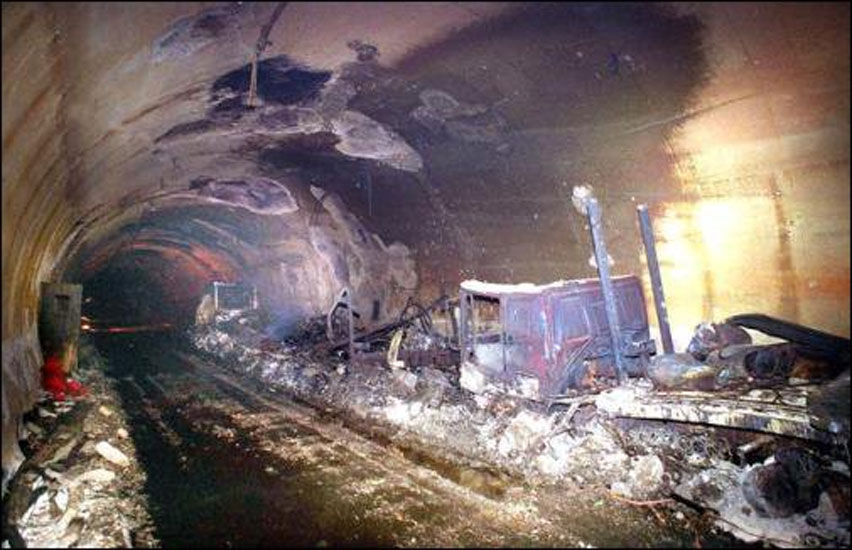
\includegraphics[scale = 0.27]{mont_blanc}
\end{enumerate}

\end{frame}

% ------------------

\subsection{Studium problemu}
\begin{frame}{Studium problemu}

\begin{enumerate}
  \item Aspekt fizyczny:
  \begin{itemize}
    \item lokalizacja,
    \item warunki krytyczne.
  \end{itemize}
  \item Charakterystyki psychologiczne i fizjologiczne:
  \begin{itemize}
    \item statystki World Health Organization,
    \item motoryka ewakuowanych,
    \item reakcja na zagrożenie.
  \end{itemize}
\end{enumerate}

\end{frame}